\documentclass[journal,twoside,web]{ieeecolor2}
\usepackage{generic}
\usepackage{cite}
\usepackage{amsmath,amssymb,amsfonts}
\usepackage{algorithmic}
\usepackage{graphicx}
\usepackage{textcomp}
\def\BibTeX{{\rm B\kern-.05em{\sc i\kern-.025em b}\kern-.08em
    T\kern-.1667em\lower.7ex\hbox{E}\kern-.125emX}}
\markboth{\journalname, VOL. XX, NO. XX, XXXX 2023}
{Author \MakeLowercase{\textit{et al.}}: Preparation of Papers for IEEE TRANSACTIONS and JOURNALS (December 2023)}
\begin{document}
\title{Preparation of Paper (Stage 1): Counting pages and fitting the figures}
\author{First A. Author, \IEEEmembership{Fellow, IEEE}, Second B. Author, and Third C. Author, Jr., \IEEEmembership{Member, IEEE}
\thanks{This paragraph of the first footnote will contain the date on 
which you submitted your paper for review. It will also contain support 
information, including sponsor and financial support acknowledgment. For 
example, ``This work was supported in part by the U.S. Department of 
Commerce under Grant BS123456.'' }
\thanks{The next few paragraphs should contain 
the authors' current affiliations, including current address and e-mail. For 
example, F. A. Author is with the National Institute of Standards and 
Technology, Boulder, CO 80305 USA (e-mail: author@boulder.nist.gov). }
\thanks{S. B. Author, Jr., was with Rice University, Houston, TX 77005 USA. He is 
now with the Department of Physics, Colorado State University, Fort Collins, 
CO 80523 USA (e-mail: author@lamar.colostate.edu).}
\thanks{T. C. Author is with 
the Electrical Engineering Department, University of Colorado, Boulder, CO 
80309 USA, on leave from the National Research Institute for Metals, 
Tsukuba, Japan (e-mail: author@nrim.go.jp).}}

\maketitle

\begin{abstract}
Distortion-product otoacoustic emissions are intermodulation products upon stimulation by two tones and reflect the nonlinear processing of sound waves within the inner ear by the so-called cochlear amplifier. Therefore, they are interpreted as diagnostic measure of the physiological state of it. Because of their very small amplitudes, current clinical systems measure one distortion product amplitude at typically some 7 frequencies and thus can be regarded as a 1D-Scan. More advanced systems record input-output functions of the distortion product amplitudes, where, however, both tones are varied in a prescribed proportion (2D-scan). When varying both tones independently, a 3D-scan giving a more complete and accurate information about the cochlea under investigation is obtained, but at the cost of vastly extended measurement time. Here, we introduce an adaptive measurement method that is shown to collect more distortion products having sufficient signal-to-noise ratio, and that in the majority of the cases leads to the identification of the so-called individually optimal stimulus level path. We compared the adaptive measurement method to a static one where the stimulus level combination are prescribed beforehand. Within a tolerance of x dB, the adaptive method found the same optimum paths than the static method within the overlap area generated by both methods, and added x\% more optimum stimulus paths where the static method failed. Ultimately, a bivariate histogram of area and density of the sampling of the optimum path shows that the adaptive method makes a better compromise between two concurring goals, as the compromise achieved is situated closer to the unachievable goal of reaching maximum density and high coverage at the same time. Thus, the adaptive method has been shown to yield a time-efficient approach to characterize the inner ear more comprehensively, which is expected to leads to more accurate diagnosis of the state of the inner ear.
\end{abstract}

\begin{IEEEkeywords}
Acoustic distortion,
auditory system,
biharmonic spline interpolation,
distortion measurement,
distortion product otoacoustic emissions,
Delaunay triangulation,
hearing,
beta skeleton
\end{IEEEkeywords}

\section{Introduction}
\label{sec:introduction}
\subsection{DPOAE, DPOAE Input-output functions and DPOAE level maps for assessment of the cochlear amplifier}
Distortion-product otoacoustic emissions (DPOAE) are sound waves generated in the nonlinear, active cochlea through the intermodulation of two-tone stimulation, with stimulus frequencies $f_1$ and $f_2$ and their stimulus levels $L_1$ and $L_2$.
DPOAE can be measured in the ear canal with a sensitive microphone.

In humans, the most pronounced DPOAEs are observed at the 3rd order intermodulation product frequency $f_{DP} = 2f_1 - f_2$.
In clinical practice, DPOAEs are used as a diagnostic tool to evaluate the function of the cochlear amplifier \cite{Ah2010}, typically with fixed frequency ratio set to approx. $f_2 / f_1 = 1.2$ to maximize response amplitude \cite{GK1990}.

Several approaches have been made to establish an optimal standard paradigm for DPOAE measurements to assess the state of the so-called cochlear amplifier.
These approaches can be described by the dimension of the parameter space \cite{Ms2002}.

The method most commonly used in clinical settings, known as a DP-Gram, measures DPOAE at a single combination of stimulus levels (often $L_2, L_1 = 55, 65$ dB SPL) for each frequency \cite{Ab2001}, and thus represents a one-dimensional scan.
The diagnostic information sought, i.e. the state of the cochlear amplifier, has a highly nonlinear and quite variable relation to the DPOAE amplitude \cite{Gr1996}, \cite{Bh2023}.
Therefore, a normative range is defined within which the amplitudes should fall if the cochlear amplifier is functioning normally.
This approach leads to a dichotomous diagnostic result, indicating whether or not the cochlear amplifier is healthy \cite{Pt1991},\cite{LM2003}.
 
A more advanced approach, DPOAE input-output (I/O) functions, uses multiple level combinations where the stimulus-tone levels are linearly related \cite{Km1998}, and thus adds a second dimension.
In this method, the DPOAE pressure responses are plotted as a function of the level of the second primary.
DPOAE input-output (I/O) functions enhance diagnostic sensitivity for detecting cochlear-amplifier-related hearing loss \cite{GK1990}, \cite{St1996}, \cite{GD2024}.
When extrapolated from semi-logarithmically scaled I/O functions, this approach provides an almost linear relationship between DPOAE threshold and pure-tone hearing threshold \cite{BJ2002}, \cite{GN2003}.
Importantly, this method allows the use of inclusion criteria that are independent of signal-to-noise ratio (SNR) thereby improving diagnostic yield and accuracy \cite{ZD2017}.

Finally, DPOAE can be sampled at a range of independent level combinations creating a three-dimensional representation in the $(L_2, L_1)$-plane, thus adding a third dimension to the data recorded per given frequency $f_2$.
 
This approach, which we refer to as DPOAE level map (LM) was initially introduced by \cite{Wh1995} and \cite{Km2000}.
DPOAE LMs of limited density or extent can also be derived from investigations on DPOAE amplitude dependence on one stimulus level alone, e.g. \cite{GK1990}, \cite{Nl2005}.
All mentioned reports used prescribed level combinations, which we refer to as static level maps (SLMs), to investigate DPOAE generation characteristics, primarily focusing on identifying group-optimal stimulus paths in the $(L_2, L_1)$-plane that lead to maximum DPOAE levels.
\cite{ZD2015a} reported on DPOAE LMs based on pulsed DPOAE using the onset decomposition (OD) method that eliminates artefacts caused by the interference of the two competing source contributions: the nonlinear-distortion component and the coherent reflection component \cite{ZD2015}.
The OD method samples the rising onset of the DPOAE signal in the time domain before the low-latency reflection component begins to interfere.
As a result, “smooth” DPOAE LMs with a clear maximum allow a more precise representation of the state of the cochlear amplifier and thus increase the diagnostic yield and accuracy \cite{ZD2015a}, \cite{ZD2020}.

\begin{figure}[ht]
\centerline{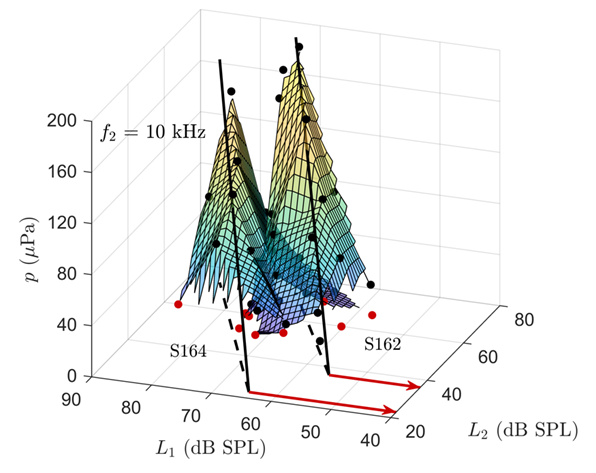
\includegraphics[width=\columnwidth]{Fig_0_v1.png}}
\caption{Two DPOAE level maps measured in different normal-hearing subjects at $f_2 = 10$ kHz.
These DPOAE LMs demonstrate cases from the study of \cite{Br2021}, where a reasonable measurement of I/O functions (black, continuous lines) cannot be achieved with one common group-optimal stimulus path in the $(L_2, L_1)$-plane, lying somewhere between the individual optimal stimulus paths (dashed black lines).
The black solid lines are referred to as ridges of the DPOAE LMs.}
\label{fig_Bdr}
\end{figure}

\subsection{DPOAE level dependence}
\label{sec1_model}
Experimental evidence from multiple studies \cite{Wh1995}, \cite{Km2000}, \cite{ZD2015a}, \cite{ZD2020}, \cite{Cr1997} indicates that DPOAE LMs in mammalians, including humans, exhibit a common characteristic, particularly at low-to-moderate stimulus levels ($L_2<50$ dB SPL).
This characteristic manifests as a distinct ridge (see Fig. \ref{fig_AMB}A) representing the maximum DPOAE amplitudes stimulated by the minimal stimulus pressure, i.e. at optimal combinations of $L_1$ and $L_2$.
The ridge’s projection onto the $(L_2, L_1)$-plane yields the level combinations that can be considered individually optimal for each ear \cite{ZD2020}.
 
The structure of DPOAE LMs can be roughly approximated by a 5-parameter model \cite{ED2017}.
This model implies that the ridge is a line in a defined $(L_2, L_1, p_{DP})$-space with parabolic cross section when DPOAEs are scaled as level ($L_{DP}=20 log_{10} (p_{DP}/20 \mu$Pa), with $p_{DP}$ being the sound pressure of the DPOAE).
The line itself is described by four parameters: ($a, b, s$ and $L_{2,EDPT}$), where $s$ is a slope in $\mathbb{R}^3$-space, $a$ the slope of the optimum path in the $(L_2, L_1)$-plane, $b$ is its $L_1$-intercept, and $L_{2,EDPT}$ is the intercept of the ridge line with the $(L_2, L_1)$-plane (edpt: estimated distortion product threshold).
The cross-section perpendicular to the ridge and the $(L_2, L_1)$-plane is provided by a 5th parameter $c$, which expands the line to a model surface with a parabolic law dependent on the level of the DPOAE, $L_{DP}$ \cite{ZD2020}.

In experimental practice, however, the ridge of a DPOAE LM is not always a straight line, the shape of the surface can deviate characteristically from the 5-parameter model, and the ridge’s position may vary significantly between individuals.
Ridge position and slope are affected by pathological but also non-pathological middle-ear transduction changes, such as minor static middle-ear pressure changes \cite{Js2005}.
Together with off-ridge points characterizing the general shape of the map, the estimated ridge representing the DPOAE I/O function may provide the clinically most important information about the DPOAE LM, as it not only allows the estimation of the hearing threshold but also represents compressive nonlinearity and allows predictions about the functional state of the cochlear amplifier independent of threshold \cite{Ab2021}.
It is, though, understood, that the regular shape of DPOAE LMs can be compromised by several factors, e.g. spontaneous otoacoustic emissions (SOAE), SNR, or time variance during measurement.

\subsection{Aim of a new method to derive DPOAE level maps}
Traditional methods, which rely on predefined, i.e. static level combinations, may fail to capture the ridge of each subject’s DPOAE response, or lead to time-consuming collection of data without any or important information.
In this article we introduce a method for adaptive DPOAE LM acquisition that is capable of autonomous exploration of a LM based on the existence of DPOAE responses and their amplitudes, and that can be tailored to different research or clinical needs.

Another aim is to assess all forms of LMs not limited to a priori assumptions about their shape as those inherent in the 5-parameter model presented in \cite{ZD2020}, specifically with regard to the derivation of a subject-specific optimal path that might not necessarily be linear in the $(L_2, L_1)$-plane.
With respect to clinical needs, the adaptive scanning algorithms investigated here might serve in future to collect DPOAE data containing the complete three-dimensional information in a most time-efficient manner.

The LM approach requires the measurement of more DPOAE than a DPOAE I/O function.
In turn, it offers two significant advantages: 1) Measuring a LM reveals the individually optimal path.
Once known, a measurement of an I/O function along this path or its derivation from the DPOAE LM provides a more accurate representation of DPOAE growth properties compared to measurements of DPOAE I/O functions along a group-optimal path (s. Fig. \ref{fig_Bdr} and \cite{ZD2020}).
Figure \ref{fig_Bdr} shows an example of maximally separated DPOAE LMs from two normal-hearing subjects which would lead to misleading results when measured with DPOAE I/O functions along one group-optimal path.
2) Characteristic shifts of the DPOAE LM and accompanying reductions of the amplitudes of their ridge are known to be produced by conductive hearing loss, i.e.
reductions of middle-ear transmission, and can therefore potentially be used for differential diagnostics of middle- and inner-ear impairments and lead to higher specificity for the diagnosis of the state of the cochlear amplifier \cite{Js2005}, \cite{Km2006}, \cite{Tu2009}, Steffen, 2017.

The here introduced adaptive measurement algorithm considerably optimizes the time required for data acquisition, making it a more efficient and reliable method for clinical diagnostics and research.

\section{Methods}
\subsection{Measurement system and calibration}
OAE measurements were conducted bilaterally using an ER-10C DPOAE probe system (Etymotic Research, Elk Grove Village, IL, USA), connected to a 16-bit analog output card and a 24-bit signal acquisition card (NI PCI 6733 and NI PCI 4472, National Instruments, Austin, TX, USA), all housed in a standard PC.
The sampling rate was set to 102.4 kHz.
Stimulus generation, data collection, and signal post-processing were carried out using a custom MATLAB toolbox ("DPAOE-Creator", version 24.2, MathWorks, Natick, MA, USA).
The sound pressure of the ER-10C speakers was determined through in-ear SPL calibration, repeated every 600 seconds.
Additional details about the calibration procedure can be found in \cite{ZD2015a}.

\subsection{DPOAE acquisition – Static level maps}
SLMs are DPOAE LMs that are recorded using predefined $(L_2, L_1)$-stimulus level combinations.
The aim is to capture the expected position of the DPOAE LM with an appropriate region around the ridge, based on the population mean parameters of the group optimum path for different frequencies.
The stimulus level combinations for SLM were adapted from \cite{ZD2020} and slightly modified especially at high stimulus levels.
The resulting grid had lateral symmetry about the expected group-mean optimum path ($L_2'$-axis, cf. Fig. \ref{fig_AMB}B), fixed distances ($10$ dB along the $L_2'$-axis, and $6$ dB along the $L_1'$-axis).
It comprises six cross sections of the expected level map with 3, 4, 5, 3, 3, 3 points per scan along the $L_1'$-axis (see Fig. \ref{fig_CNT}, red pattern).
The position of the grid is defined by $(L_{2,MIN} , L_{1,MIN})$, s. Fig. \ref{fig_CNT}, for values,  s. Sec. V, Table 1), which were based on the experience from previous experiments \cite{Br2021} to optimize data yield in normal-hearing subjects.

\subsection{DPOAE acquisition – Adaptive level maps}
Adaptive LMs (ALMs) are defined as DPOAE LMs that are procedurally generated to increase the efficiency of DPOAE acquisition.
After measuring a prescribed starting point, the algorithm selects the next stimulus level combinations based on the configuration of assessed data and their relation to an expected LM shape.
This is accomplished by comparison of accepted DPOAE, i.e. those with $SNR \ge 10$ dB, with the 5-parameter model defining the a priori expectance of a LM shape.

An initial level combination (i.e. $p_1^1$ on Fig.\ref{fig_AMB}B) is chosen in a frequency-dependent manner with$L_{2,START} = 55 dB$ for $f_2 < 4 kHz$, 60 dB for $f_2 < 8 kHz$, and $65 dB$ for larger $f_2$, while $L_1$ is chosen to lie $6 dB$ below the group-optimal level according to \cite{ZD2020} (see Table I, Sec. V  I).
 In principle, all adaptive methods described in the following can be utilized stand-alone or in conjunction, depending on the particular clinical or research task.
We subdivide the adaptive methods into two groups.

\begin{figure*}
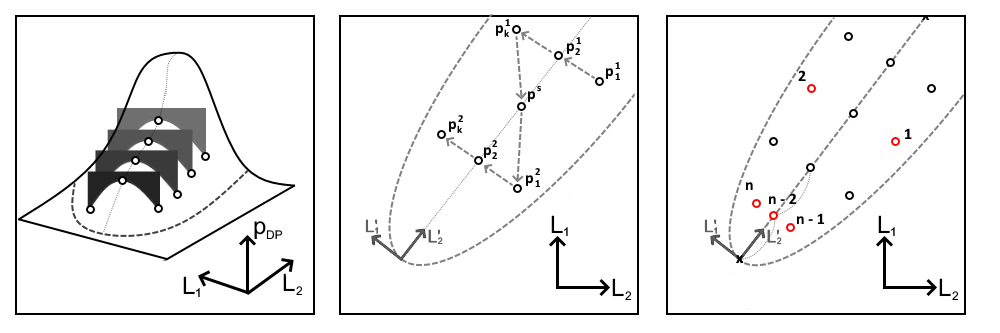
\includegraphics[width=\textwidth]{Fig_ALM_ModelBased} %,height=4cm
\caption{Model-based algorithms to identify the ridge of DPOAE LMs: A: Model surface of an ideal DPOAE LM, described via perpendicular scans, illustrating the expected structure of a typical DPOAE LM.
B: Ridge estimator method.
To minimize the number of points per measurement, this method employs two ridge scans ($p^1_i$ and $p^2_i$) and one intermediate point $p^s$.
Ideally, it samples seven points to estimate all major characteristics of the DPOAE LM.
C: Ridge follower method.
This method strongly relies on the estimated DPOAE LM surface and is used to enhance the resolution of points along the ridge.
It requires a minimum of three points per scan (the ridge point and one point on either side) and provides a prescribed overall amount of scans perpendicular to the ridge.}
\label{fig_AMB}
\end{figure*}

The first group of ALM acquisition methods relies on the expected shape of a DPOAE level map, i.e., it uses a priori knowledge as discussed in Section I.C, and shown in Fig. \ref{fig_AMB}A.
Two methods belong to the a priori group: the so-called ridge estimator and ridge follower.
To simplify the description of the ALM methods, we refer to a $(L_2’, L_1’)$-plane which is rotated such that the projection of the ridge onto the $(L_2, L_1)$-plane aligns with the $L_2'$ axis (s. Fig. \ref{fig_AMB}B).
The angle of the rotation corresponds to the group mean parameter a of the 5-parameter model (s. Sec. \ref{sec1_model}, and \cite{ZD2020}).

The ridge estimator \cite{ED2017} is utilized to verify the presence of the presumed DPOAE LM and to roughly estimate model surface properties.
The algorithm is comprised of three steps – two ridge scans and one intermediate point (see Fig. \ref{fig_AMB}A for ridge and Fig. \ref{fig_AMB}B for illustration of the ridge estimator algorithm):
\begin{algorithmic}[1]
\STATE An initial ridge scan $p_k^1$ samples the presumed ridge along $L_1'$ starting from an initial level combination $p_1^1$ and aims to detect its maximum to prove the existence of a ridge.
Every single ridge scan might take up to $k$ DPOAE amplitudes or points (here: $k=4$), limited by a pre-defined region of interest (ROI).
The ROI might be tailored to specific tasks, but typically will contain an upper limit for $L_2$ and $L_1$ to avoid acoustic overstimulation and/or technical distortions (here: $95$ dB SPL).
Sampling during a ridge scan has two modes: 1) if there are no accepted DPOAE amplitudes or points, the $L_1'$ increment is set to $10$ dB, 2) if the acquired DPOAE adhere to the predefined acceptance criteria (based on SNR, s. Sec. \ref{sec2_study}), the $L_1'$ increment is set to $6$ dB.
If the detected DPOAE amplitude $p_{DP}$ decreases after two successful measurements, the $L_1'$ increment is switched to be negative.
Once three DPOAE have been accepted, the maximum is determined by solving a quadratic equation to their levels.
If four attempts fail to determine a ridge, an additional scan is deployed on half distance between the existing scan and upper ROI boundaries.
\STATE Once a maximum within a ridge scan is detected, an intermediate point $p^s$ is sampled to estimate individually the slope of the ridge.
This point is positioned based on the assumed frequency dependence of the slope s of the group mean optimal path, a (\cite{ZD2020}, their Table I) and on the typical background noise levels – such that it is expected to fall on half distance between the first scan and the location where the prescribed minimum SNR for an accepted DPOAE would be obtained.
In this study, $SNR_{MIN}$ was set to $10$ dB.
\STATE After the slope of the DPOAE LM ridge is individually computed, a starting point for the 2nd low-level scan perpendicular to the ridge is set at a $L_2'$ where a $SNR = SNR_{MIN} + 12$ dB is expected.
This value was chosen empirically as a compromise between the goals to obtain valid DPOAEs at low stimulus-levels and to avoid measuring neighbouring off-ridge points without achieving the required SNR.
After measuring an initial point, the second scan $p_k^2$ is performed in the same manner as $p_k^1$ (see step 1).
\end{algorithmic} 

The second acquisition method of the \textit{a priori} group is the "ridge follower".
This method involves two recurrent steps (see Fig.\ref{fig_AMB}C) aimed at enhancing the resolution of the DPOAE data along the ridge:
\begin{algorithmic}[1]
\STATE For any existing singular point on the ridge (e.g., $p^s$ in Fig.\ref{fig_AMB}B), two satellite points are assigned on either side of the ridge.
There can also exist other incomplete scans because the presumed ridge which is calculated by the 5-parameter model, may have shifted during the procedure.
Therefore, after recalculation of the model, no point within a scan is situated within $\pm1$ dB of the calculated ridge, a new ridge point is measured.
This choice was done in order to ensure that a growth function along a linear path can be constructed without interpolation.
\STATE If no singular points are left, a new point (s.
Fig. \ref{fig_AMB}C: $n – 2$) is positioned on the ridge.
The longest empty interval, either between the ROI boundaries and the nearest point or between existing points along the ridge, is identified, and the new point is placed by bisecting the interval.
\end{algorithmic} 

A second group of "data-based" acquisition methods was implemented, relying solely on the already existing points based on Delaunay triangulation \cite{LS1980} referred to as"polygonal search method" (PSM).
The PSM and terms used in the following are borrowed from graph theory.
It comprises two cases – the general and the expansive case.

\begin{figure*}
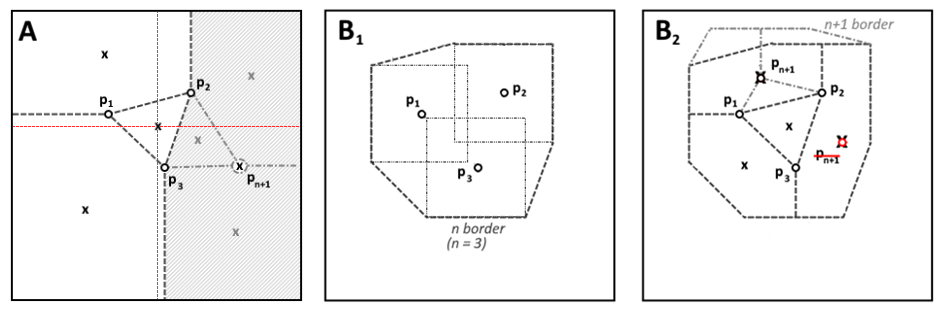
\includegraphics[width=\textwidth]{Fig_ALM_DataBased} %,height=4cm
\caption{Data-based algorithm to identify DPOAE LM without a priori assumptions on its shape.
A situation may arise where certain points have been measured, but the model surface cannot be accessed.
In such cases, an algorithm is used that systematically searches for data points in the $(L_2, L_1)$ level depending on the SNR.
A: The general case of the Polygonal Search Method (PSM) splits the ROI into smaller polygons and takes the centre of mass ($p_{n+1}$, marked as cross) of the biggest polygon (gray hatched area) to be measured next.
B: An expansion case of PSM is a stricter version of general case, which bases its prediction only on “accepted” points.
It generates the boundary (n border), by using square regions of vicinity around “accepted” points.
C: Inside the boundary, the general case of the PSM (A) is applied to find the next point to be measured.}
\label{fig_ADB}
\end{figure*}

In the general case of the PSM (see Fig.\ref{fig_ADB}A), any existing points with all kind of DPOAE amplitudes within the boundaries of the ROI are considered.
The data-based algorithm consists of the following steps:
\begin{algorithmic}[1]
\STATE All points which have already been measured (continuous-line circles in Fig.\ref{fig_ADB}A, $p_{1...3}$), are processed with a Delaunay triangulation function (matlab function \textit{delaunayTriangulation(P)}) that generates triangle polygons, based on those and defined via vertices coordinates list and triangular face connectivity list (\cite{LS1980}; see their Appendix B).
\STATE To construct polygons adjacent to boundaries of the ROI, the vertices of the alpha shape of all acquired points, i.e. the circumference of the set of triangles, are connected to the boundaries of the ROI according to the minimum-distance principle (vertical and horizontal lines in Fig.\ref{fig_ADB}A).
To prevent edge clustering, the $(L_2, L_1)$-plane is divided into four sections by two orthogonal lines (see red dashed lines in Fig.\ref{fig_ADB}A) intersecting at the centre of mass of the alpha shape.
Points can only be connected to a boundary located in the same section.
\STATE Once all connections between the points and the boundaries are established, the updated connectivity list contains all non-overlapping polygons within the ROI.
The largest polygon (see gray polygon in Fig.\ref{fig_ADB}A) is selected and its centre of mass is chosen as the next measurement point.
\end{algorithmic} 

If PSM is applied without prior data, the subdivision of the $(L_2, L_1)$-plane (step 2) begins in a pre-described initial point and creates four different polygons.
Following this step, the method continues with the aforementioned steps.

In the expansion case of the PSM, only points with accepted DPOAE amplitudes are taken into account and the ROI is redefined based on those points in every step.
For each accepted point, neighbouring points defining a group are identified by their distances with $\delta L_2 \le 10 dB$, $\delta L_1 \le 15$ dB.
Around these points, a square-shaped region of pre-defined size is built (here: $20 \times 20 dB$), and their common circumference is yielding a polygon, which describes the new ROI (s. Fig .\ref{fig_ADB}B, dashed line).
Following these rules, more than one ROI can appear.
The final step is to employ the general case for all groups simultaneously, meaning that the largest polygon identified in any group generates the next point (s. Fig. \ref{fig_ADB}C).
The expansion case has the advantage to constrain the ROI to an area where the probability might be deemed high to lead to accepted DPOAE.

\subsection{Study design and subjects}
\label{sec2_study}

The pilot study, validating the adaptive algorithm for DPOAE LM acquisition, included three normal-hearing subjects (age: 27, 31 and 37 years old).
All three subjects were classified as normal-hearing as all pure-tone thresholds were better than $20$ dB hearing level (dB HL) for frequencies between 1 and 8 kHz.

DPOAE LMs were recorded bilaterally at 14 frequencies ranging from 1 to 14 kHz ($f_2 = 1, 1.5, 2, 3, 4, 5, 6, 8, 9, 10, 11, 12, 13, 14$ kHz), yielding 84 independent data sets.
The stimulus and recording sequence are based on a time-interlaced multi-frequency acquisition technique (Zelle, 2014).
21 level combinations per frequency were chosen, each of which averaged over 44 ensembles comprising four blocks with appropriate phase shifts to apply the PTPV technique.
Within a block of length of 0.18 seconds, 7 frequencies are presented in a time-interlaced manner; the whole measurement including intermittent calibrations took approximately 25 minutes.
For each measured DPOAE amplitude, we performed sorted averaging, estimated the noise floor and, if SNR exceeds 10 dB, the corresponding point was considered accepted.
The noise floor was estimated as the root-mean-square of the difference between two subsets of the underlying segments from the DPOAE recording in a 50-ms time interval centred on the DPOAE response.
The subsets were created by averaging two sets of interlaced PTPV ensembles, each of which contained four consecutive segments with suitable phase variations to cancel the stimulus pulses.


\begin{figure}[ht]
\centerline{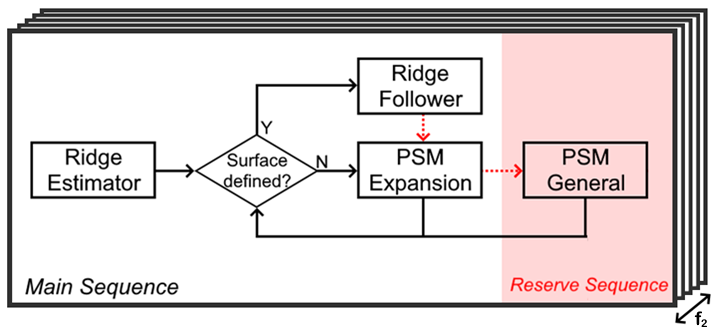
\includegraphics[width=\columnwidth]{Fig_Sequence.png}}
\caption{Adaptive acquisition workflow: Black arrows – regular sequence, red arrows – exception sequence (if measurement at prescribed point is not possible for any reason).}
\label{fig_SQS}
\end{figure}

The sequence of measurements used in this study is depicted in Fig.\ref{fig_SQS}.
After assessment of pure-tone thresholds using a Békésy tracking method (for details: \cite{Br2021}) , DPOAE are acquired with ALM followed by SLM in a subsequent visit after 1-2 months.
During ALM acquisition (see Section II.C), the sequence of \textit{a priori} and \textit{data-based} acquisition methods is followed independently for each frequency stimulated within a block.
The sequence is organized so, that after completion of the ridge estimator, the model is fitted to all previously assessed DPOAE amplitudes after each measurement.
The 5-parameter model is accepted if the following criteria are met: $r^2 > 0.8, \sigma \le 10$, where $r$ is the correlation coefficient between DPOAE amplitudes and the 5-parameter model fitted to them, and $\sigma $ is standard error of the model parameter $L_{2, EDPT}$ (\cite{ZD2020}; see Section I B).
If these criteria are satisfied, the ridge follower algorithm complements the level map, if not, the PSM expansion method is initiated.


The study was approved by the Ethics Committee of the University of Tübingen and   was conducted in accordance with the Declaration of Helsinki for human experiments.

\subsection{Post-processing and analysis}
\label{sec2_pproc}

\subsubsection{Connectivity-based analysis of acceptance rate and coverage}
To compare and analyse SLM and ALM without relying on the surface shape produced by the DPOAE, we use quantities that are present in each measurement: number of all acquired points ($N_{all}$), number of points with accepted DPOAE amplitudes ($N_{acc}$), and the area of the alpha shape ($S$) of $N_{acc}$ (s. Fig. \ref{fig_CNT}).
Additionally, for post-processing here we restrict the connectivity list such, that it does not have triangles with edges larger than $18$ dB, to minimize the influence from extrapolation artefacts, which might take place in next subsection.

\begin{figure}[ht]
\centerline{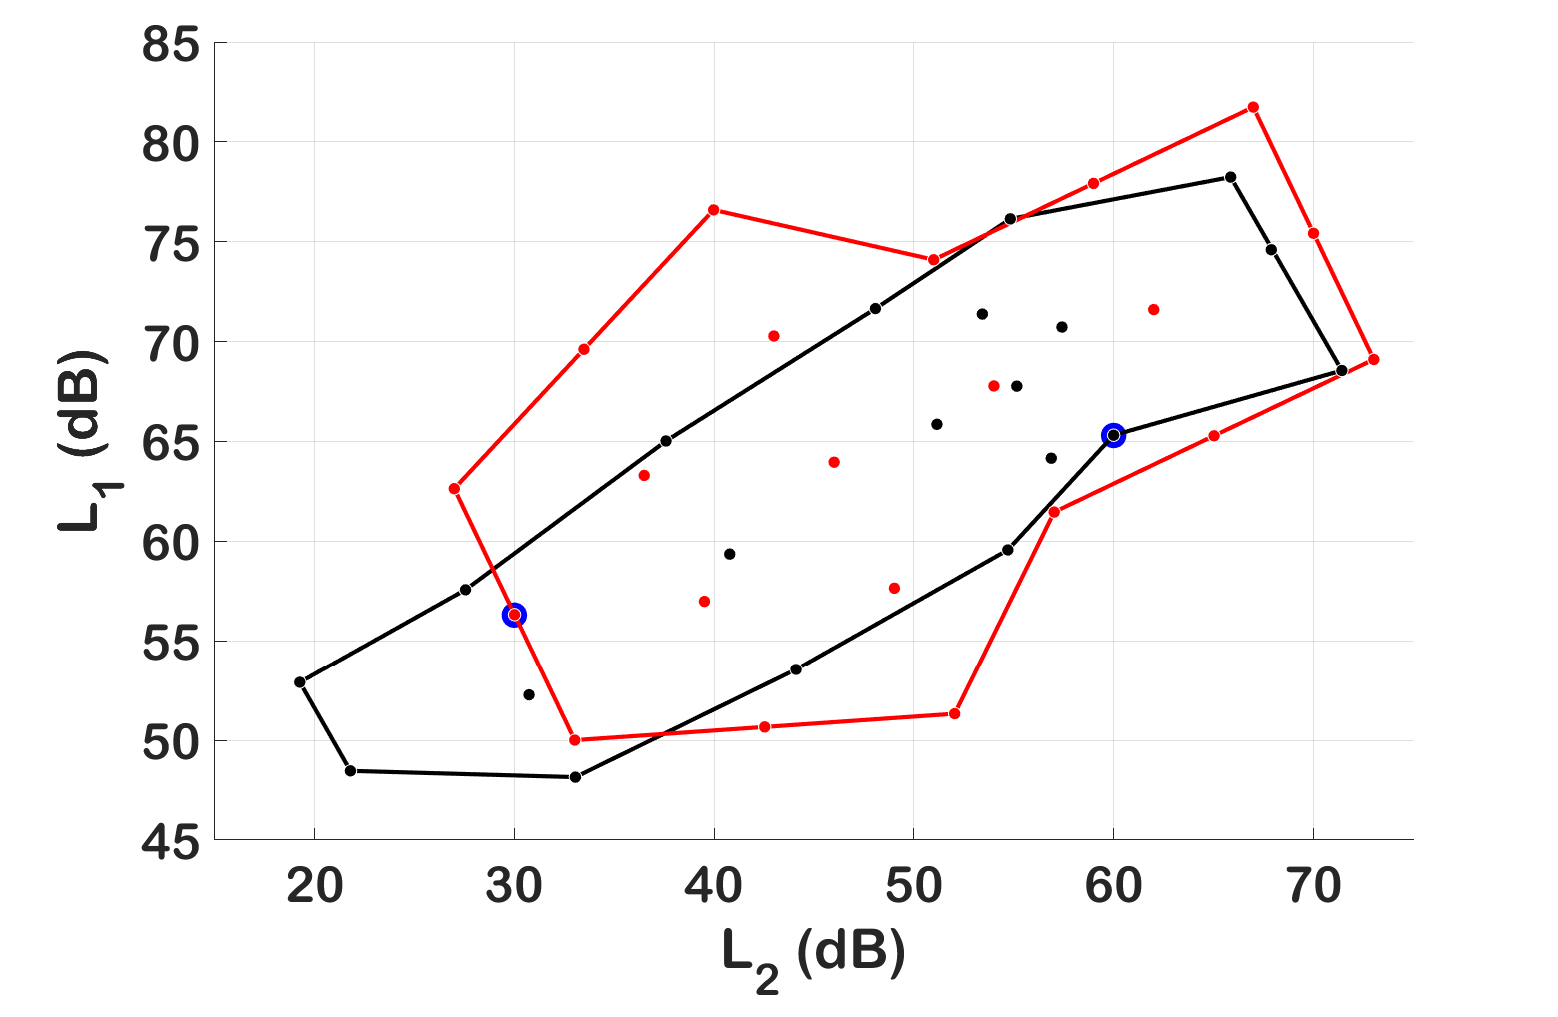
\includegraphics[width=\columnwidth]{Fig_3_connectivity.eps}}
\caption{Accepted points and their correspondent alpha shapes: adaptive (black) and static (red) level maps.
Initial points for both approaches are highlighted with blue circles.
An ideal scenario where all points meet the acceptance criteria, and the level maps do not clip to the ROI boundaries.}
\label{fig_CNT}
\end{figure}

Time efficiency of an LM measurement is defined here as the ratio of accepted points to all acquired points $(N_{acc}/N_{all})$.
The second metric is used to assess a “goodness” of coverage.
Together with $S$, the areal density of the points with accepted DPOAE amplitudes $(\rho = N_{acc} / S)$ creates a $(\rho, S)$-space, where the main underlying assumption is, that there exists an ideal LM with ideal values, i.e.
$(\rho _{max}, S_{max})$, where $\rho _{max}$, $S_{max}$ are the maximum values of these variables across all LMs (here 6 ears x 14 frequencies x 2 methods).
In this context, any reduction in Nacc leads to a value below one.
Similarly, any dispersion over a larger area S in the $(L_2, L_1)$-plane leads to a value below one.
The latter criterion $\rho < 1$  is here taken as an indicator of loss of information.

\subsubsection{Analysis of LM features}
First, the accepted points, acquired with SLM and ALM, are interpolated using biharmonic splines \cite{DZ2011}.
For ridge identification, the measured LM is transformed into a gradient field.
A simplified version of the Dijkstra algorithm \cite{Di1959} is used to trace the path with the least inclination from the peak towards lower values.
The customized algorithm includes the following simplifications: it operates on a predefined mesh graph, only allows movement towards lower or equal $L_2$ values from the initial point, has an open end instead of searching for a distant endpoint, and considers only neighboring nodes of the mesh.
To reduce oscillations and enhance stability, additional weighting is applied to the gradient field based on two rules: 1) nodes with $L_2$ lower than initial point (close-range interaction bias $= 0.995$) and 2) nodes, which are closer to the line connecting the initial point to the closest local minimum on gradient field, have their weight additionally modified (long-range interaction bias $= 0.9$).


To compare LM shapes obtained via different methods, we need a common measure that incorporates all the evaluated data.


This is achieved by applying a joint polynomial fit to the ridges obtained by the SLM and the ALM method.
Each ridge is fitted to its own polynomial with $k$ characteristic low-order terms and iterative $n-k$ shared higher-order components.
The order of the polynomial is incremented by 1 and is limited by $k = 1$, $n_{max} = 15$.


\begin{align}
\begin{cases}
p_{n} x_{\alpha}^n&+p_{n-1} x_{\alpha}^{n-1}+\cdots+p_{k+1} x_{\alpha}^{k+1} \\
&+\alpha_k x_{\alpha}^{k}+\alpha_{k-1} x_{\alpha}^{k-1}+\cdots+\alpha _0 x_{\alpha}^0-y_{\alpha} =0 \\
p_{n} x_{\beta}^n&+p_{n-1} x_{\beta}^{n-1}+\cdots+p_{k+1} x_{\beta}^{k+1} \\
&+\beta_k x_{\beta}^{k}+\beta_{k-1} x_{\beta}^{k-1}+\cdots+\beta _0 x_{\beta}^0-y_{\beta} =0 \\
& \vdots 
\end{cases}
\label{eq1}
\end{align}

The k-fold cross-validation is used to prevent overfitting, where amount of folds is selected dynamically based on size of data (with minimum four and maximum ten folds).
When one of the lines is considered to be overfitted, then previous state is taken as a result.

A common ridge is then determined by fitting the remaining free components using the previously identified higher-order terms.
The final step is to calculate the distances of points to the joint fit of the ridges of SLM and ALM methods (see Fig.\ref{fig_BLK}).

\section{Results}

\begin{figure*}
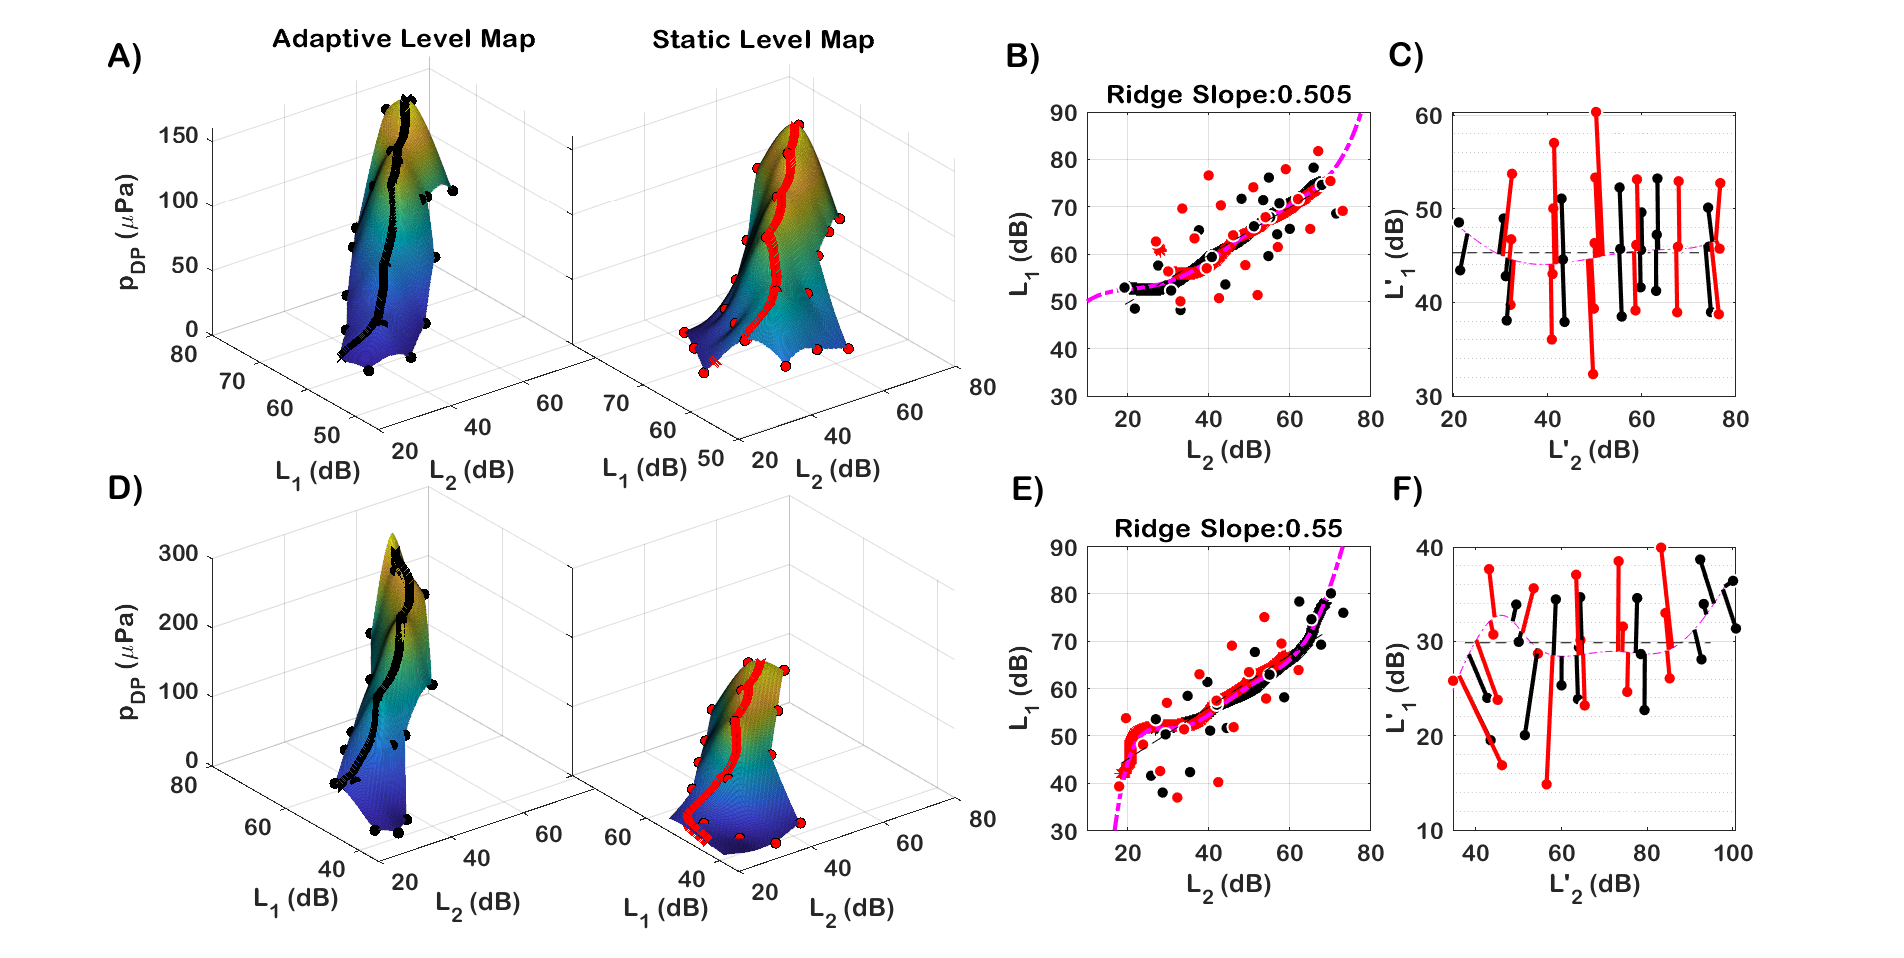
\includegraphics[width=\textwidth]{Fig_5_assembly2.eps} %,height=4cm
\caption{Comprison of feature identification with SLM and ALM method. A, D: A level map interpolated with biharmonic splines and its ridge, estimated using the "ridge searcher" method.
B, E: Estimated ridges from the LMs in A, D and a general ridge derived through iterative polynomial fitting of these two ridges.
C, F: Distances between the general ridge and measured points for both maps.
A–C: represent a nearly ideal case (S345, 4 kHz), where the data are centered to the sampling grid for both methods, whereas D–F show a more typical result of LM acquisition, where the sampled area differs more clearly between both methods. (S345, 1 kHz).\\ Black color – ALM, Red color – SLM.}
\label{fig_BLK}
\end{figure*}

\subsection{Qualitative features of the interpolation and ridge comparison method}
Fig. \ref{fig_BLK}A-C and Fig. \ref{fig_BLK}D-F show two examples of LMs pairs obtained with the adaptive (black curve) and the static (red curve) method.
The upper example (Fig. \ref{fig_BLK}A) illustrates an acquisition of a nearly ideal level map.
For both, the ALM and the SLM, all measured points met the SNR criterion (only points, passing the SNR criterion, are connected by the mesh illustrating the surface in (Fig. \ref{fig_BLK}B)).
The interpolation method used introduces rippling along the ridge, which does not reflect the true shape of the level map, and should be considered as an artefact resulting from the spline interpolation method between two experimentally obtained points.
The black and the red line designate the result of the ridge search algorithm (see Section II.E).
In the upper example (Fig. \ref{fig_BLK}A–C), the ridge lines cut almost always through the central points of the sampling grid for both methods, whereas for the bottom example, this is the case only for the ALM method. Nonetheless, the ridges are almost identical where the data overlap.


An example where SLM and ALM methods have led to slightly different area coverage is shown in Fig. \ref{fig_BLK}D.
Fig.~\ref{fig_BLK}B and E show the projection of the identified ridges and the stimulus level pairs of accepted points onto the $(L_2, L_1)$-plane.
In the upper example, the ridges of both, ALM and SLM, align closely and correspond to almost straight lines.
However, in Fig. \ref{fig_BLK}E,  the area covered by the SLM method is shifted toward lower $L_2$ values, especially at high levels. Nonetheless, the ridges identified by both methods are very close to each other in the area where both methods contribute.
The projection of both ridge identifications onto the $(L_2, L_1)$-plane shows that the ALM technique succeeds in capturing the ridge on its center line of the sampling grid in both examples.

\subsection{Acceptance rate and time efficiency}
Fig.~\ref{fig_EFF}A shows the acceptance rate ($N_{acc}/N_{all}$), representing the portion of points that passed the $10$ dB SNR criterion, across all six ears, dependent on frequency.
In general, ALM measurements resulted in a greater number of accepted points at most frequencies, the exceptions being 3, 12, and 13 kHz.
Fig. \ref{fig_EFF}B shows the histogram of the acceptance rate within a single LM across all frequencies and all ears.
ALM show in $36\%$ of all LMs an acceptance rate of $\ge 0.95$, i.e. 20 out of 21 or all points which have been tested passed the SNR criterion, while the correspondent figure for SLM was only $10\%$.
The median of the acceptance rate was 0.62 and 0.78 for SLM and ALM indicating that ALM is more effective in setting stimulus levels to achieve DPOAE signals with SNR $\ge10$ dB compared to SLM.

\begin{figure}[ht]
\centerline{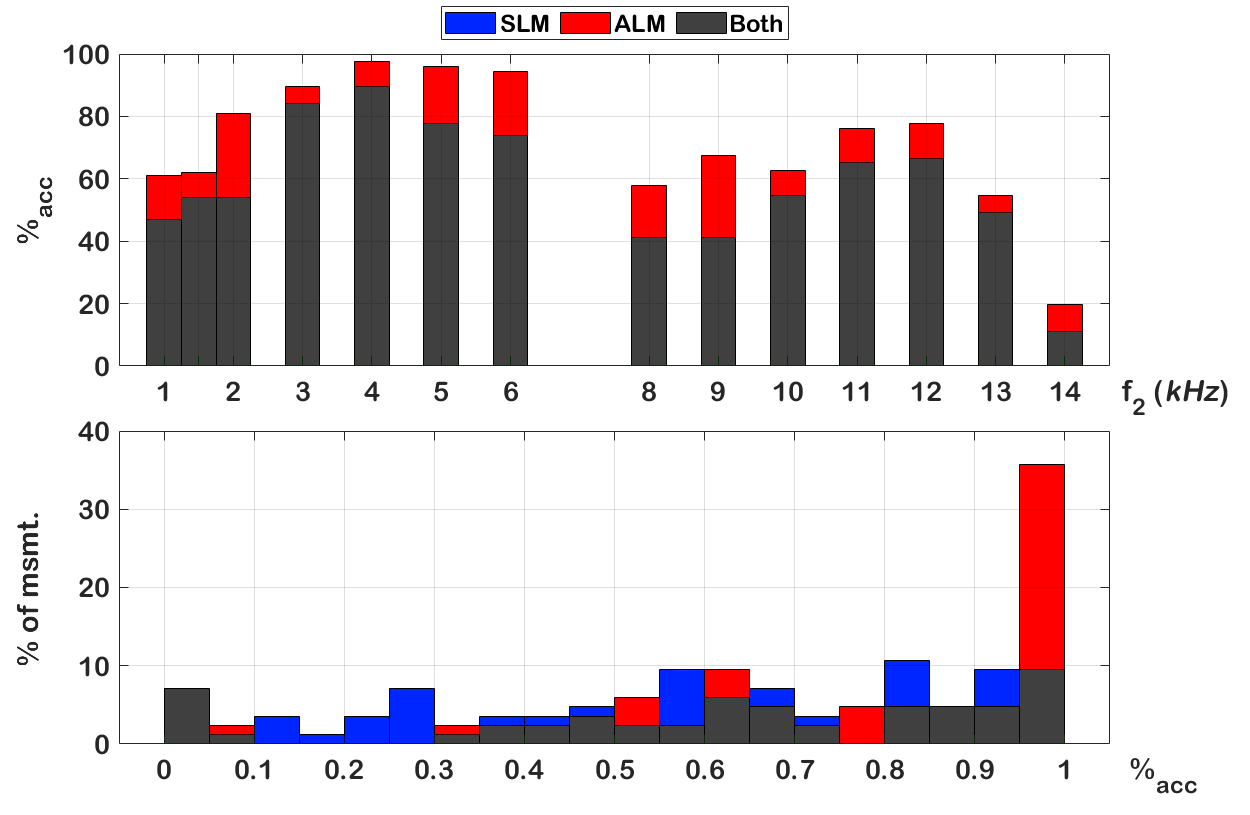
\includegraphics[width=\columnwidth]{Fig_Efficiency_v3.png}}
\caption{A) Share of accepted points over frequencies for all ears.
B) Distribution of percentage of accepted points per single LM measurement for all frequencies and ears.
Black color shows the method with the smaller or equal share. The ALM method contributes more accepted DPOAE determinations at all frequencies (panel A), and it succeeds in 36\% of the cases to provide 95–100\% valid DPOAE, i.e. in theses cases at least 20/21 DPOAE measurements within a given LM were reaching the SNR criterion, as compared to only 10\% for the SLM method.}
\label{fig_EFF}
\end{figure}

Overall, we obtained 1020 accepted DPOAE amplitudes with SLMs and 1258 accepted DPOAE amplitudes with ALMs, indicating a $23\%$ increase in quantitative output.

\subsection{Coverage of DPOAE LMs}
To compare the relative performance of both methods, we performed a joint analysis of the area, defined by the alpha shape corresponding to the accepted points, and their $(L_2, L_1)$-density (see Section II.E).
Both values $(\rho, S)$ are min-max normalized in linear space and converted to log space (see \eqref{eq2}):
\begin{equation} log(\rho) = log(\frac{\rho - \rho_{min}}{\rho_{max} - \rho_{min}}); log(S) = log(\frac{S - S_{min}}{S_{max} - S_{min}}), \label{eq2}\end{equation}
where the minimum and maximum values are determined separately for each LM.
Thus, in linear space, $\rho$ and $S$ cannot attain values of $> 1$, or equivalently their logarithm cannot become $> 0$.
Therefore, a deviation of any of either parameters towards “$-\infty$” designates a loss of information.

\begin{figure*}
\centering
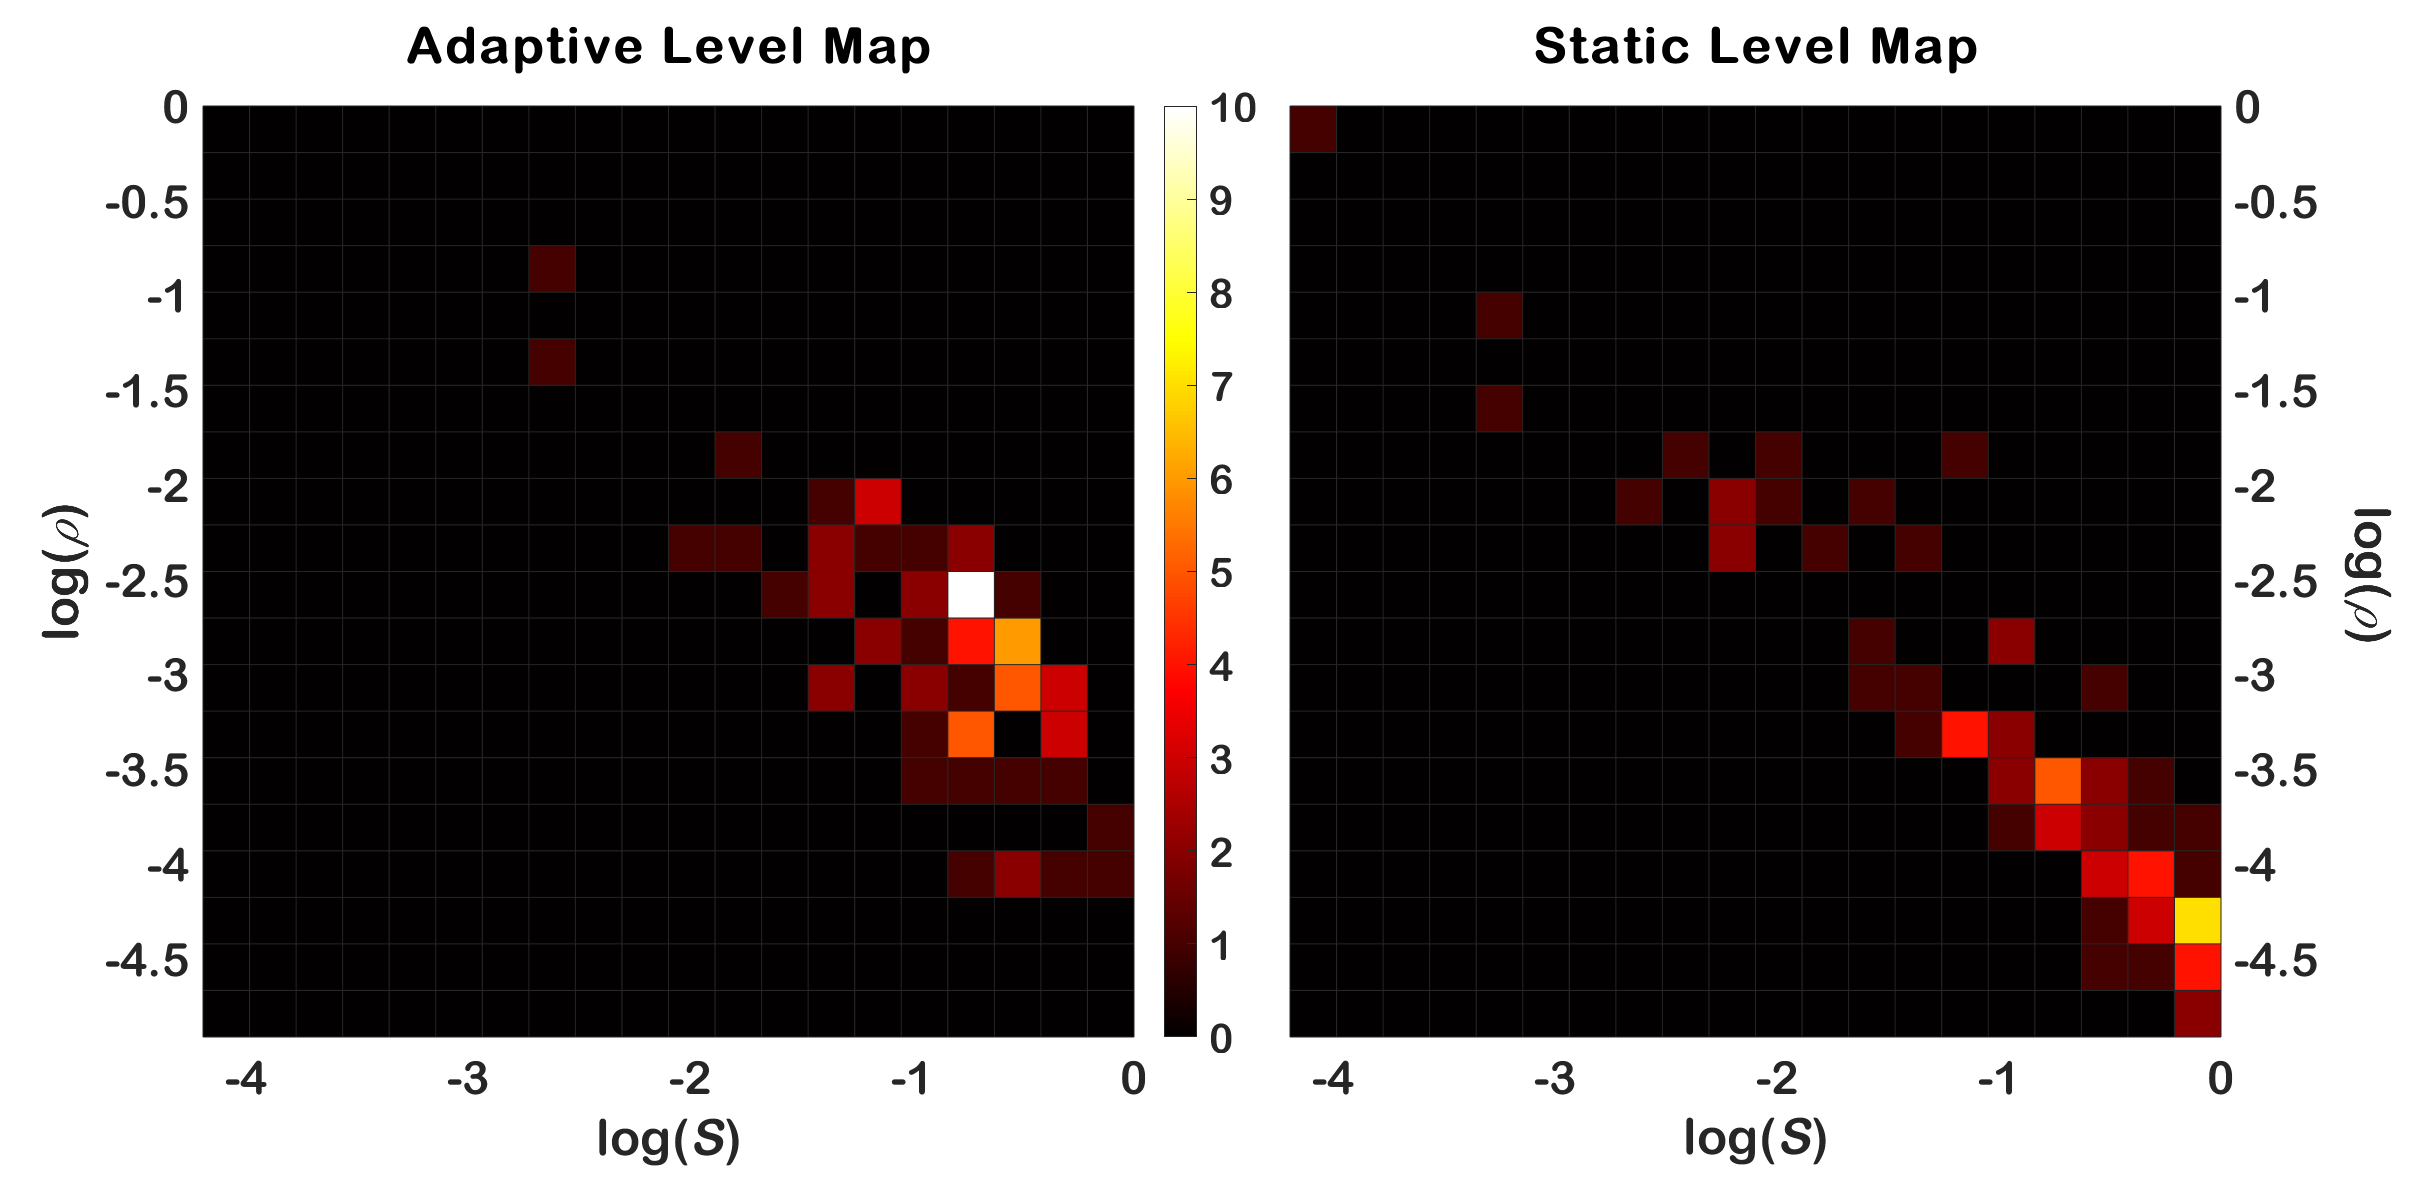
\includegraphics[width=.8\textwidth]{Fig_8_Coverage_sameClim.eps} %,height=4cm
\caption{Bivariate histogram of level map areas and their corresponding point density.
This histogram is representing the qualitative aspect of LM properties which were encountered oin this study.
There is an assumed ideal LM with largest area and density, which is located in $(0, 0)$, but cannot be obtained with the given amount of $N_{all}$.
The colour scheme ranges from black through red to white.
Higher colour intensity designates higher amount of counts.}
\label{fig_TGT}
\end{figure*}

Fig. \ref{fig_TGT} shows a bivariate histogram of area and density for the obtained LMs, with the left panel representing ALM, and the right panel representing SLM.
The majority of measurements acquired with the ALM method (cluster around the brightest square) is shifted closer towards $(0, 0)$, compared to those obtained by the SLM method.
This shift suggests that ALMs prioritizes point density over area coverage, resulting in an improved resolution of the LMs close to the ridge.


\begin{figure}[ht]
\centerline{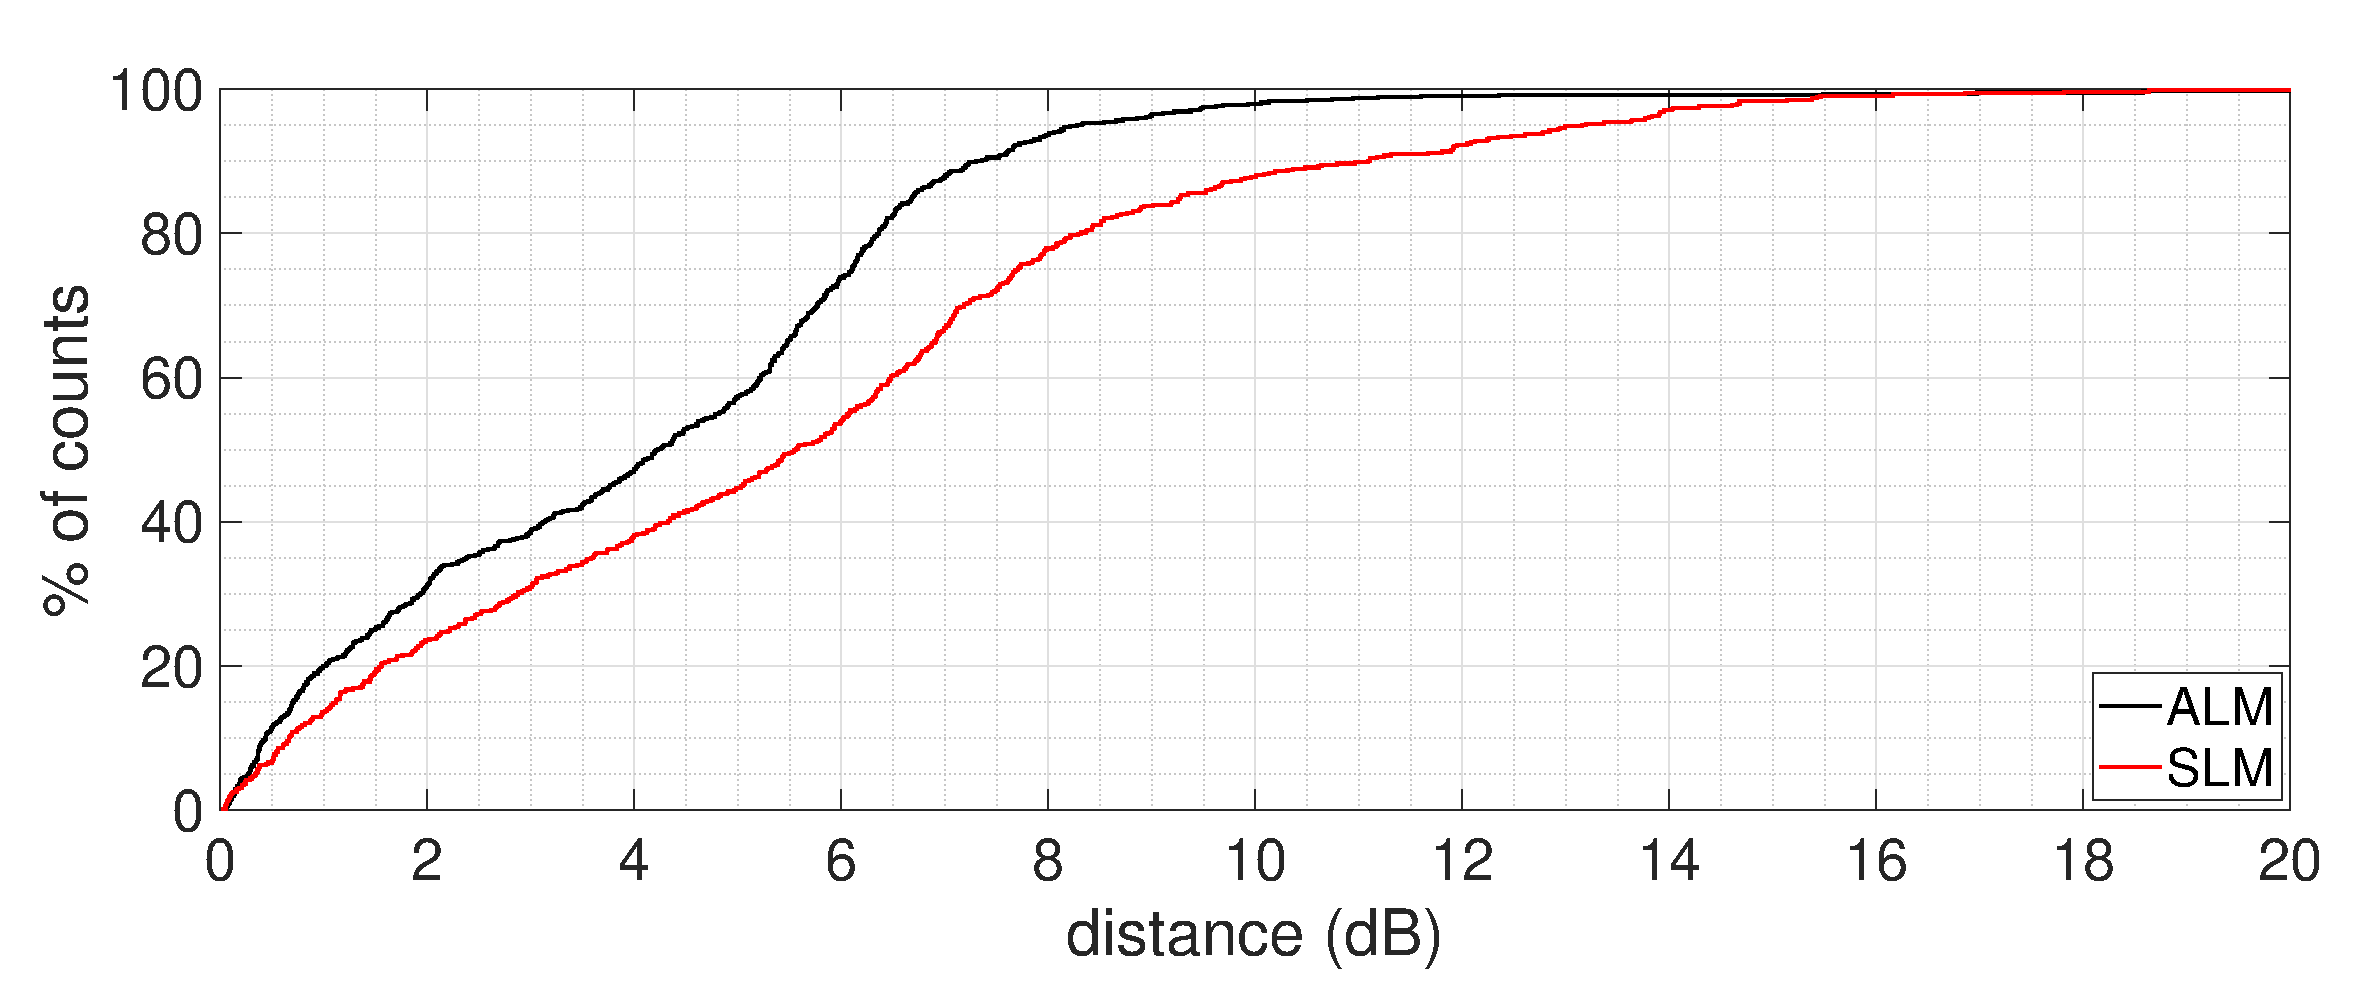
\includegraphics[width=\columnwidth]{Fig_9_Cumula.eps}}
\caption{Empirical cumulative distribution function of the distances between the estimated ridge and measured points for all LMs where both, ALM and SLM, passed the acceptance criteria for identifying a ridge (each ridge length must be more than $12dB$ and both - ALM and SLM ridges - must exist)}
\label{fig_CDF}
\end{figure}

Fig. \ref{fig_CDF} shows the cumulative distribution of the distance of the $(L_2, L_1)$-coordinates of accepted points from the ridge.
For ALM, 74\% of the accepted points lie within $6$ dB from the ridge, compared to only 54\% for SLM.
Moreover, in the static methods, more than 20\% of points are over $8$ dB away from the ridge.
Taking a typical level map cross section given by $L_{DP} =-0.12 \Delta L_1'^2$ (Eq. 4 and Tbl. I in \cite{ZD2020}), $8$ dB off ridge suggests already a relative loss in SNR of $7.7$ dB, compared to only $4.3$ dB for $6$ dB distance.

\begin{figure}[ht]
\centerline{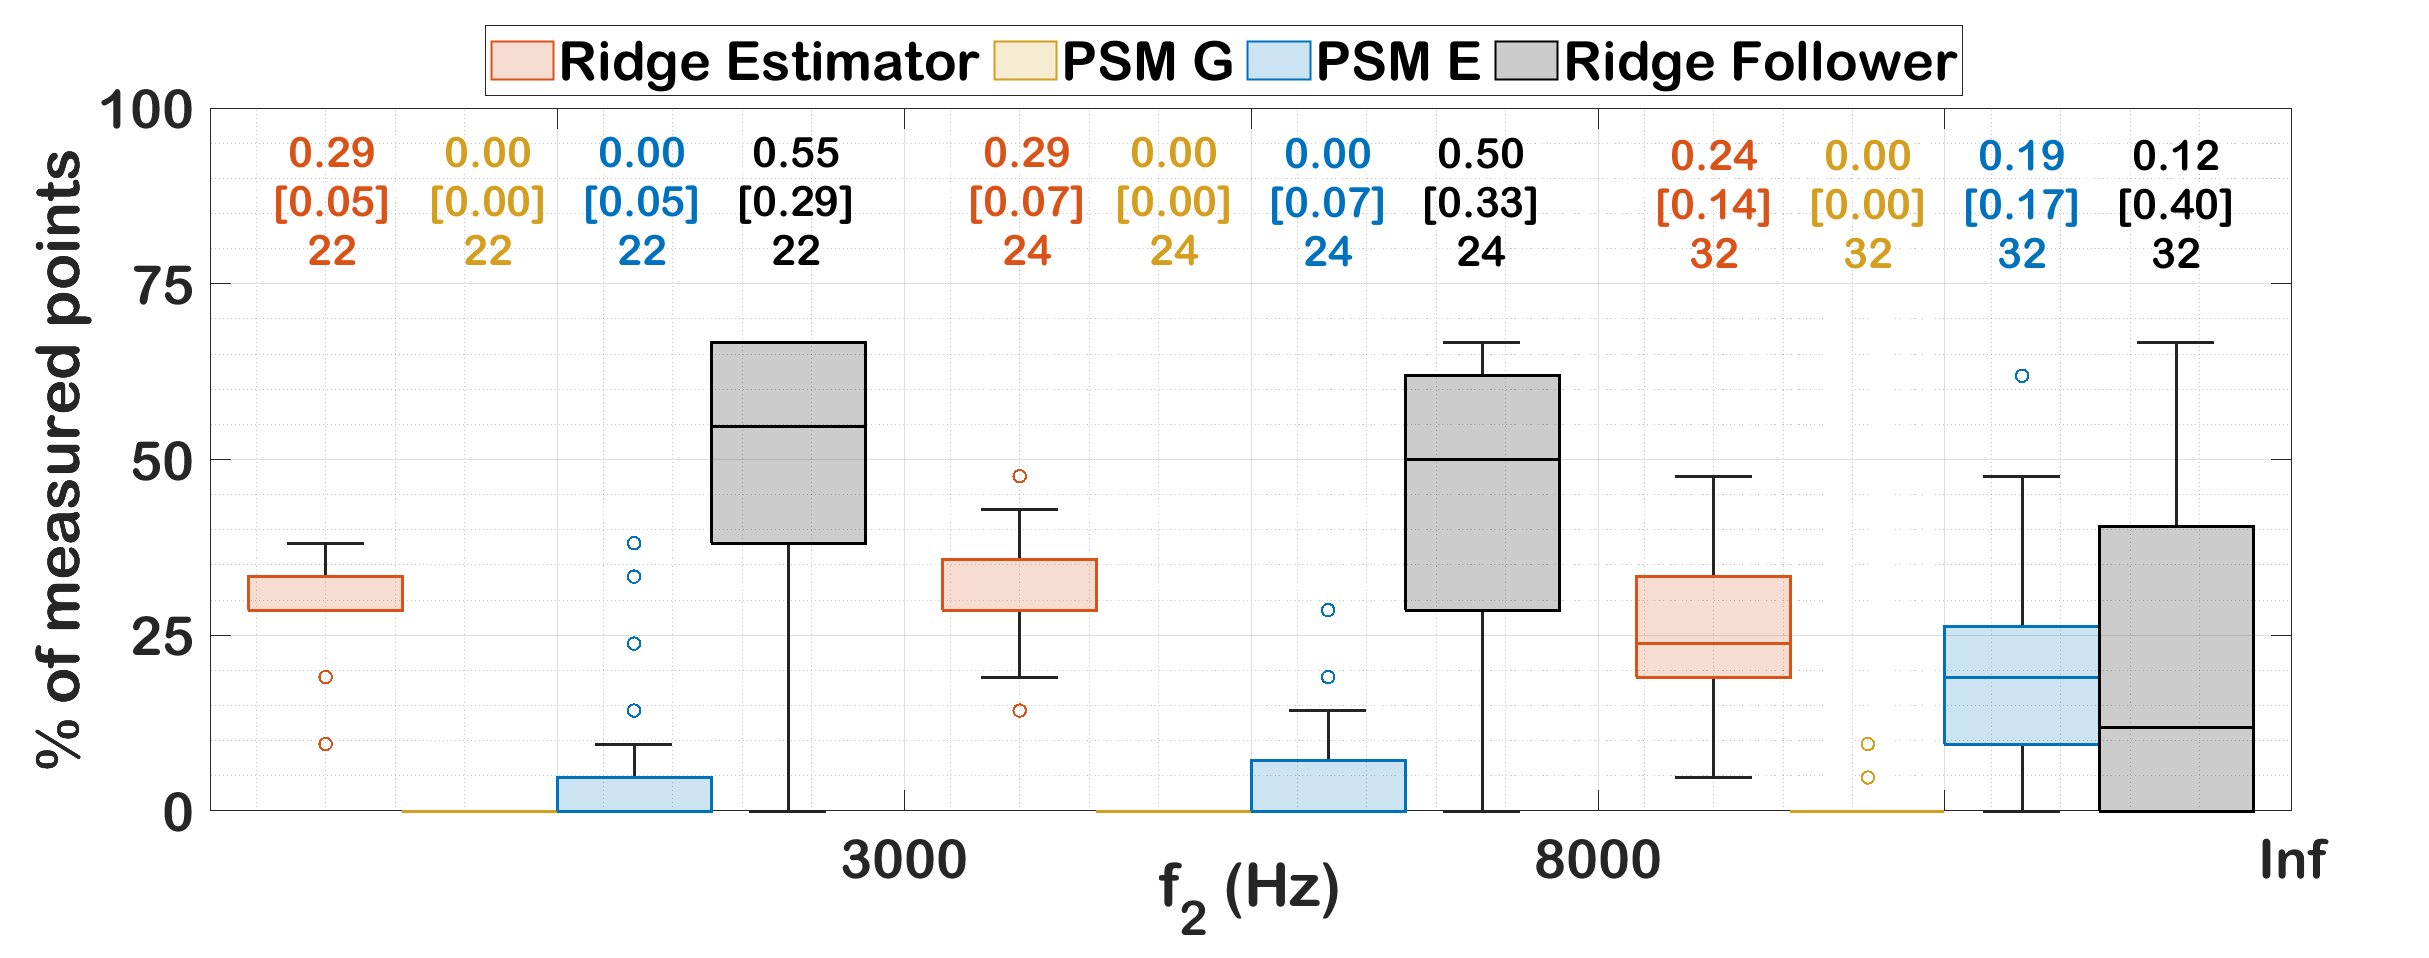
\includegraphics[width=\columnwidth]{Fig_10_Boxplots.eps}}
\caption{Median, interquartile ranges, and range of the share of accepted DPOAE within a level map which was obtained by the four adaptive acquisition methods, grouped into three frequency ranges.
Numbers above the box-whisker plots are: Median, interquartile range, and amount of datasets containing at least 6 accepted DPOAE, which were 78 out of 84 possible datasets.}
\label{fig_BXP}
\end{figure}

Fig. \ref{fig_BXP} shows the performance of the four adaptive acquisition methods in the implementation used here, given as statistics of the ratio of accepted points collected by a single method to all accepted points within a given LM.
For the both lower frequency ranges, judged by the median, more than 80\% of the accepted points were successfully acquired by the a priori methods (ridge estimator and ridge follower), whereas the adaptive acquisition workflow (Fig. \ref{fig_SQS}) only seldom needed to invoke the data-based algorithms.
On the contrary, for the high-frequency range, as judged by the median, only 36\% of the accepted points were contributed by the a priori methods, whereas the data-based methods gained importance and contributed 19\%.

\section{Discussion}
This study pursued two major goals: First, design and evaluate an adaptive level-map acquisition method that is able sample the LM where DPOAE with acceptable SNR can be obtained.
The second goal was to develop and investigate a method for characterization and comparison of LMs obtained by different methods without limiting the comparison to a priori assumptions on their shape such as the 5-parameter model.

\subsection{Method advantages and drawbacks}
In most or probably all medical imaging techniques, the acquisition of the data, even when not measured simultaneously in a single capture, is not designed to depend on the data themselves.
At best, the region of interest is planned in advance to meet the needs of an individual patient.
For DPOAE-acquisition, a simultaneous acquistion is largely not realizable because of the nonlinear interactions inside the cochlea, and, for a single parameter set (frequencies, levels, etc.), the necessary recording time can already take 1 minute depending on the DPOAE's level, thus rendering acquisition of 3D information extremely time consuming.

Therefore, the ALM method presented here are designed to extract only the features deemed relevant from the resulting LM while avoiding as much as possible to measure at stimulus levels where sufficient SNR cannot be reached within the prescribed time.
To address this, we employed a two-stage search sequence, consisting of pattern recognition (a priori) and exploratory (data-based) methods.
The a priori methods have proven to work well at all frequencies, but especially at frequencies at and below 8 kHz where they contributed more than 80\% of the DPOAE with acceptable SNR.

Here, the exploratory methods have been used in the case that the a priori methods failed to identify a LM of the expected structure (as judged by the 5-parameter model).
 The concept of the exploratory methods might be seen analogous to the one shown in Fig.\ref{fig_AMB}A-B of  \cite{Ch1997}, where the sampling grid of a pattern recognition task first covers the entire image and then becomes finer in areas to capture the relevant features more accurately.
While theirs and our methods differ in their implementation and execution, they share a common structure and topology, as both methods use a simplified beta skeleton of the data, which is a subset of the Delaunay triangulation that can be reconstructed into a polygonal surface \cite{Ep1998}.
This dynamic approach allowed us to obtain useful data in the case that the a priori methods did fail where they could have been successful (this appeared in x cases ), or a number of valid DPOAE that could be used for diagnosis even though they do not allow a valid model fit.

\subsection{Time concern}
It might be instructive to consider two cases, a typical clinical and a typical research application.
In a routine clinical application, more than some 7 to 9 points per level map will probably be undesirable, because with a typical amount of 6–8 test frequencies, extrapolation of the figures given in Sec. \ref{sec2_study} would lead to a measurement time of 3min35' to 6min8' in the current implementation.
According to our estimation, by further optimization of the implementation, i.e. reducing measurement time where in the current implementation excessively high SNR are obtained, the measurement time could be reduced to below 4 min, what would be clinically practicable.
The added use of the technique would then be: 1) Avoiding incorrect DPOAE growth properties due to applying individually wrong level combinations, 2) Obtaining an additional independent parameter, i.e. the relative position of the LM's ridge along the $L'_1$-coordinate, which is a marker for conductive hearing loss.

If we consider a basic research aim as, for instance, the characterization of individual LMs dependent on the frequency ratio $f_2/f_1$, one easily ends up with substantial measurements times: for instance, if one sets out for testing 5 different frequency ratios at 7 frequencies, and reduces the number of points per LM to 12, we find approximately 35' overall measurement time (calculated from the overall measurement time of 25' and the number of points per LM and frequencies used in this study, s. Sec. \ref{sec2_study}.
The estimate depends on the mean frequency because of the pulse length definition.).
This is a considerable measurement time which easily grows to more than an hour with more demanding requirements on sampling density of the different dimensions of interest, and at such high measurement times, the 12\% gain in accepted DPOAE compared to SLM is highly useful (s. Sec. III B).



\subsection{LM post-processing and analysis}
To analyse LMs of different origins, we devised a toolset that largely avoids a priori assumptions, the only exception being a weak a priori assumption about its direction (Sec. \ref{sec2_pproc}), in the sense that the algorithm for the identification of the vector of least gradient, i.e. the ridge, preferes the direction toward low $L_2$.
The method generally worked stable and was able to identify all ridges where the 5-parameter model also achieved an acceptable fit .
The metrics for evaluation of SLM and ALM method performance, that is, number of accepted DPOAE, coverage, and resolution of the optimum path, all show that the ALM technique worked well and superior to the SLM method.
Of course, some of these metrics, especially what we call here the resolution of the optimum path, include partially sort of a self-fulfilling prophecy.
By taking 6 dB as sampling step along the $L'_1$ direction, the points gathered, if successfully, will be closer to the ridge compared to the SLM where the grid raster converted to an $L'_1$-value was 8 dB .
On the other hand, the SLM has to make a compromise: If the grid raster becomes too fine, the number of LMs where the ridge cannot be identified due to its interindividual variation in position relative to the $L'_1$-axis, will rise, or, otherwise, a fourth and fifth line of samples has to be recorded along the complete range of $L_2$-values.
In this respect, the SLM method was already well optimized, having 4 and 5 samples orthogonal to the ridge at two low-to-moderate $L_2$ stimulus levels, in order to reduce the probability of recording valid data without being able to fit the 5-parameter model to it.

With any reasonable amount of  level combinations to be recorded, one has to make a compromise with regard to the resolution along and orthogonally to the ridge.
Here, by our desgin of the ALM method, we chose basically an optimal grid of 3x7 points to characterise the ridge, if the a priori methods would be successful, which often was the case.
The representation of the algorithm in the $(\rho, S)$-space is a suitable method to visualize the quality of any such method, because the compromise between two conflicting goals, a high point density and a high covered area is determined in 2D space.
Especially here, the ALM method shows that a clearly better compromise has been achieved, and that much more of the LM acquisitions are positioned in higher proximity to the unachievable goal, i.e., reaching maximum density and high coverage at the same time.


\section{Conclusion (WORDS LIMIT = 300)}
Here, we have introduced an adaptive method to acquire DPOAE LMs. DPOAE LMs are of clinical interest, because I/O functions derived from LMs are basically not affected by the choice of a group-optimal stimulus level path, and because conductive (i.e., middle-ear) loss might potentially be detectable, enabling a differential diagnosis that distinguishes it from inner-ear loss \cite{Js2005}, \cite{Ma2017}. On the other hand, LMs are important from a basic-research perspective for a more complete characterization of the distortion generation process. The comparison of these to the output of models of cochlear mechanics then can serve to evaluate and improve such models.
The ALM technique has produced maps which are qualitatively equivalent to SLMs within the region of overlap, as judged by the identified ridges as well as by the rms-pressure difference between these maps within the overlap region. Simultaneously, the ALM data yield is considerably higher, in our study with normal-hearing subjects overall by 23\% and has led to NUM\% more DPOAE with acceptable SNR in case where the lowest stimulus level with acc. DPOAE was $\ge 40$ dB SPL. {\bf (? - checking)}
Ultimately, the bivariate histogram of area and density has shown that the ALM makes a clearly better compromise between the both concurring goals, and that the compromise achieved is situated closer to the unachievable goal, i.e., reaching maximum density and high coverage at the same time.


\bibliographystyle{IEEEtran}
\bibliography{references}

\begin{IEEEbiography}[{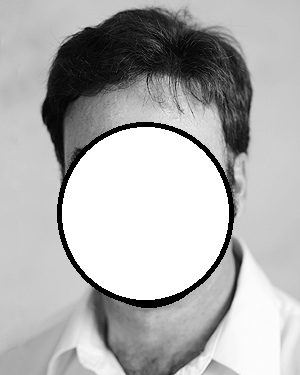
\includegraphics[width=1in,height=1.25in,clip,keepaspectratio]{author1.png}}]{First A.
Author} (M'76--SM'81--F'87) and all authors may include 
biographies.
Biographies are often not included in conference-related
papers.
This author became a Member (M) of IEEE in 1976, a Senior
Member (SM) in 1981, and a Fellow (F) in 1987.
The first paragraph may
contain a place and/or date of birth (list place, then date).
Next,
the author's educational background is listed.
The degrees should be
listed with type of degree in what field, which institution, city,
state, and country, and year the degree was earned.
The author's major
field of study should be lower-cased.


The second paragraph uses the pronoun of the person (he or she) and not the 
author's last name.
It lists military and work experience, including summer 
and fellowship jobs.
Job titles are capitalized.
The current job must have a 
location; previous positions may be listed 
without one.
Information concerning previous publications may be included.

Try not to list more than three books or published articles.
The format for 
listing publishers of a book within the biography is: title of book 
(publisher name, year) similar to a reference.
Current and previous research 
interests end the paragraph.
The third paragraph begins with the author's 
title and last name (e.g., Dr.\ Smith, Prof.\ Jones, Mr.\ Kajor, Ms.\ Hunter).

List any memberships in professional societies other than the IEEE.
Finally, 
list any awards and work for IEEE committees and publications.
If a 
photograph is provided, it should be of good quality, and 
professional-looking.
Following are two examples of an author's biography.
\end{IEEEbiography}

\begin{IEEEbiography}[{
\includegraphics[width=1in,height=1.25in,clip,keepaspectratio]{author2.png}}]{Second B.
Author} was born in Greenwich Village, New York, NY, USA in 
1977.
He received the B.S.
and M.S.
degrees in aerospace engineering from 
the University of Virginia, Charlottesville, in 2001 and the Ph.D.
degree in 
mechanical engineering from Drexel University, Philadelphia, PA, in 2008.

From 2001 to 2004, he was a Research Assistant with the Princeton Plasma 
Physics Laboratory.
Since 2009, he has been an Assistant Professor with the 
Mechanical Engineering Department, Texas A{\&}M University, College Station.

He is the author of three books, more than 150 articles, and more than 70 
inventions.
His research interests include high-pressure and high-density 
nonthermal plasma discharge processes and applications, microscale plasma 
discharges, discharges in liquids, spectroscopic diagnostics, plasma 
propulsion, and innovation plasma applications.
He is an Associate Editor of 
the journal \emph{Earth, Moon, Planets}, and holds two patents.


Dr.
Author was a recipient of the International Association of Geomagnetism 
and Aeronomy Young Scientist Award for Excellence in 2008, and the IEEE 
Electromagnetic Compatibility Society Best Symposium Paper Award in 2011.

\end{IEEEbiography}

\begin{IEEEbiography}[{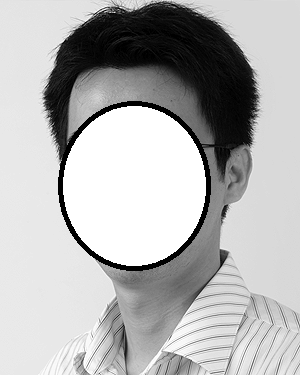
\includegraphics[width=1in,height=1.25in,clip,keepaspectratio]{author3.png}}]{Third C. Author, Jr.} (M'87) received the B.S. degree in mechanical 
engineering from National Chung Cheng University, Chiayi, Taiwan, in 2004 
and the M.S.
degree in mechanical engineering from National Tsing Hua 
University, Hsinchu, Taiwan, in 2006.
He is currently pursuing the Ph.D.

degree in mechanical engineering at Texas A{\&}M University, College 
Station, TX, USA.

From 2008 to 2009, he was a Research Assistant with the Institute of 
Physics, Academia Sinica, Tapei, Taiwan.
His research interest includes the 
development of surface processing and biological/medical treatment 
techniques using nonthermal atmospheric pressure plasmas, fundamental study 
of plasma sources, and fabrication of micro- or nanostructured surfaces.


Mr.
Author's awards and honors include the Frew Fellowship (Australian 
Academy of Science), the I.
I.
Rabi Prize (APS), the European Frequency and 
Time Forum Award, the Carl Zeiss Research Award, the William F.
Meggers 
Award and the Adolph Lomb Medal (OSA).
\end{IEEEbiography}

\end{document}
